\documentclass[11pt]{article}

\usepackage[margin=1in]{geometry}
\usepackage[T1]{fontenc}
\usepackage[utf8]{inputenc}
\usepackage{lmodern}
\usepackage{microtype}
\usepackage{amsmath,amssymb,mathtools,bm}
\usepackage{booktabs,tabularx,array}
\usepackage{xcolor}
\usepackage{hyperref}
\usepackage[most]{tcolorbox}
\usepackage{tikz}
\usepackage{tikz-3dplot}
\usepackage{pgfplots}
\usepackage{enumitem}
\usepackage{float}
\usepackage{caption}
\usepackage{fancyhdr}
\usepackage{titlesec}

\pgfplotsset{compat=1.18}
\usetikzlibrary{arrows.meta,calc,positioning,patterns,decorations.pathreplacing,intersections,3d,backgrounds,shadings}

\hypersetup{
  colorlinks=true,
  linkcolor=blue!60!black,
  urlcolor=blue!60!black,
  citecolor=blue!60!black,
  pdftitle={Chapter 23. Stokes Theorem and the Divergence Theorem}
}

\setlength{\headheight}{14pt}
\setlength{\parindent}{0pt}
\setlength{\parskip}{0.62em}
\setlist[itemize]{topsep=2pt,itemsep=2pt}
\setlist[enumerate]{topsep=2pt,itemsep=2pt}

\titleformat{\section}{\large\bfseries\color{blue!55!black}}{\thesection}{0.6em}{}
\titleformat{\subsection}{\normalsize\bfseries\color{blue!45!black}}{\thesubsection}{0.6em}{}

\pagestyle{fancy}
\fancyhf{}
\lhead{Chapter 23. Stokes Theorem and the Divergence Theorem}
\rhead{\thepage}
\renewcommand{\headrulewidth}{0.4pt}

\definecolor{chapterblue}{HTML}{1F5AA6}
\definecolor{chapterteal}{HTML}{168A8F}
\definecolor{chapterorange}{HTML}{D9822B}
\definecolor{chaptergreen}{HTML}{2D8A4E}
\definecolor{chapterpurple}{HTML}{6B4EAA}
\definecolor{chapterred}{HTML}{B23B3B}
\definecolor{softblue}{HTML}{EAF3FF}
\definecolor{softgreen}{HTML}{EAF8EF}
\definecolor{softorange}{HTML}{FFF4E6}
\definecolor{softpurple}{HTML}{F3EEFF}
\definecolor{softred}{HTML}{FFF0F0}
\definecolor{softgray}{HTML}{F6F7F9}

\newtcolorbox{overviewbox}{
  enhanced,breakable,colback=softblue,colframe=chapterblue,
  boxrule=0.7pt,arc=2mm,left=2mm,right=2mm,top=1mm,bottom=1mm
}
\newtcolorbox{bridgebox}[1][]{
  enhanced,breakable,colback=softpurple,colframe=chapterpurple,
  title={#1},fonttitle=\bfseries,boxrule=0.7pt,arc=2mm
}
\newtcolorbox{goalbox}{
  enhanced,breakable,colback=softgreen,colframe=chaptergreen,
  title=Learning goals,fonttitle=\bfseries,boxrule=0.7pt,arc=2mm
}
\newtcolorbox{theorembox}[1][]{
  enhanced,breakable,colback=softblue,colframe=chapterblue,
  title={#1},fonttitle=\bfseries,boxrule=0.8pt,arc=2mm
}
\newtcolorbox{tipbox}[1][]{
  enhanced,breakable,colback=softgreen,colframe=chaptergreen,
  title={#1},fonttitle=\bfseries,boxrule=0.7pt,arc=2mm
}
\newtcolorbox{importantbox}[1][]{
  enhanced,breakable,colback=softred,colframe=chapterred,
  title={#1},fonttitle=\bfseries,boxrule=0.7pt,arc=2mm
}
\newtcolorbox{examplebox}[1][]{
  enhanced,breakable,colback=white,colframe=chapterblue,
  title={#1},fonttitle=\bfseries,boxrule=0.7pt,arc=2mm
}
\newtcolorbox{warningbox}[1][]{
  enhanced,breakable,colback=softorange,colframe=chapterorange,
  title={#1},fonttitle=\bfseries,boxrule=0.7pt,arc=2mm
}

\newcommand{\R}{\mathbb R}
\newcommand{\curl}{\nabla\times}
\newcommand{\diverg}{\nabla\cdot}
\newcommand{\ii}{\mathbf i}
\newcommand{\jj}{\mathbf j}
\newcommand{\kk}{\mathbf k}
\newcommand{\vr}{\mathbf r}
\newcommand{\vn}{\mathbf n}
\newcommand{\vF}{\mathbf F}
\newcommand{\dd}{\,d}

\begin{document}

\begin{center}
  {\LARGE\bfseries Chapter 23. Stokes Theorem and the Divergence Theorem\par}
  \vspace{0.3em}
  {\large Boundary measurements, local derivatives, circulation, and flux\par}
\end{center}

\begin{overviewbox}
The previous chapters introduced vector fields, line integrals, curl, divergence, surface integrals, and flux. This chapter puts those ideas together into two central global theorems of vector calculus:
\[
\oint_{\partial S}\vF\cdot d\vr
=
\iint_S(\nabla\times\vF)\cdot\vn\,dS
\]
and
\[
\iint_{\partial E}\vF\cdot\vn\,dS
=
\iiint_E\nabla\cdot\vF\,dV.
\]
The first theorem says that \textbf{circulation around a boundary} can be measured by \textbf{curl through a surface}. The second says that \textbf{outward flux through a closed boundary} can be measured by \textbf{divergence inside the solid}.
\[
\boxed{\text{global boundary measurement}=\text{accumulated local derivative inside}.}
\]
\end{overviewbox}

\begin{bridgebox}[Bridge to applied mathematics, statistics, and AI]
Stokes theorem and the Divergence theorem teach a powerful modeling habit: do not only compute pointwise quantities. Ask how local behavior accumulates globally. This perspective reappears in conservation laws, PDEs, diffusion models, probability flux, score-based generative models, graph flows, and numerical methods on grids and meshes.
\end{bridgebox}

\begin{goalbox}
After reading this chapter, you should be able to:
\begin{enumerate}
  \item state Stokes theorem and identify the surface, boundary curve, orientation, curl, and circulation;
  \item state the Divergence theorem and identify the solid, closed boundary surface, outward normal, divergence, and flux;
  \item choose between a direct line integral, a direct surface integral, Stokes theorem, and the Divergence theorem;
  \item use orientation rules correctly;
  \item recognize the common structure behind the Fundamental Theorem of Calculus, Green's theorem, Stokes theorem, and the Divergence theorem;
  \item verify these theorems numerically in simple examples;
  \item explain how these ideas support conservation laws, flow models, and computational applied mathematics.
\end{enumerate}
\end{goalbox}

\section{The family of fundamental theorems}

The one-variable Fundamental Theorem of Calculus says
\[
\int_a^b f'(x)\,dx=f(b)-f(a).
\]
The left side accumulates a derivative over an interval. The right side measures boundary values at the endpoints:
\[
\text{total change inside}=\text{boundary difference}.
\]
For vector calculus, intervals become curves, surfaces, and solids.

\begin{center}
\begin{tabularx}{\textwidth}{>{\bfseries}lXX}
\toprule
Theorem & Interior quantity & Boundary quantity\\
\midrule
Fundamental Theorem of Calculus & derivative on an interval & endpoint values\\
Fundamental Theorem for Line Integrals & gradient along a curve & potential values at endpoints\\
Green's theorem & curl or divergence over a plane region & circulation or flux around boundary\\
Stokes theorem & curl through a surface & circulation around boundary curve\\
Divergence theorem & divergence inside a solid & flux through closed boundary surface\\
\bottomrule
\end{tabularx}
\end{center}

\begin{tipbox}[One guiding sentence]
Stokes theorem converts \textbf{boundary circulation} into \textbf{surface curl}, while the Divergence theorem converts \textbf{closed-surface flux} into \textbf{solid divergence}.
\end{tipbox}

\begin{figure}[H]
\centering
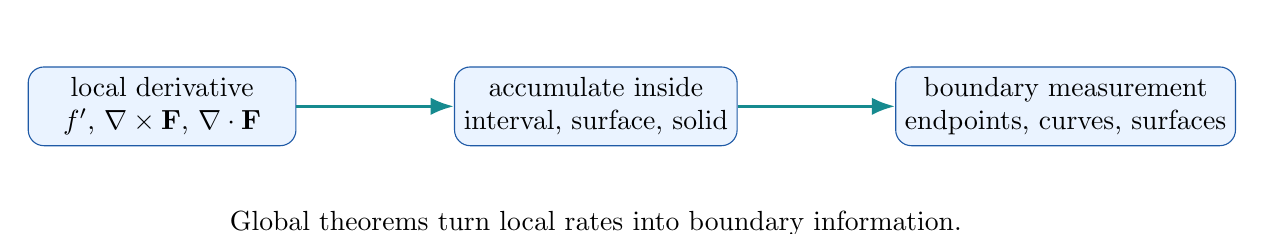
\begin{tikzpicture}[node distance=1.5cm,>=Latex]
\tikzset{box/.style={draw=chapterblue,rounded corners=2mm,fill=softblue,align=center,minimum width=3.4cm,minimum height=1.0cm}}
\node[box] (local) {local derivative\\$f'$, $\curl\vF$, $\diverg\vF$};
\node[box,right=2.0cm of local] (accum) {accumulate inside\\interval, surface, solid};
\node[box,right=2.0cm of accum] (boundary) {boundary measurement\\endpoints, curves, surfaces};
\draw[->,very thick,chapterteal] (local) -- (accum);
\draw[->,very thick,chapterteal] (accum) -- (boundary);
\node[below=0.7cm of accum,align=center] {Global theorems turn local rates into boundary information.};
\end{tikzpicture}
\caption{The common structure behind the global theorems of calculus.}
\end{figure}

\section{Orientation and boundary direction}

Orientation is the most common source of mistakes in this chapter. For a surface $S$, choosing a unit normal vector $\vn$ gives an orientation. If $S$ has a boundary curve $\partial S$, then the orientation of $\partial S$ is determined by the right-hand rule:
\begin{itemize}
  \item point the thumb of your right hand in the direction of $\vn$;
  \item your curled fingers give the positive direction around $\partial S$.
\end{itemize}
For a closed surface $\partial E$, such as a sphere or the boundary of a box, the standard orientation is \textbf{outward}.

\begin{figure}[H]
\centering
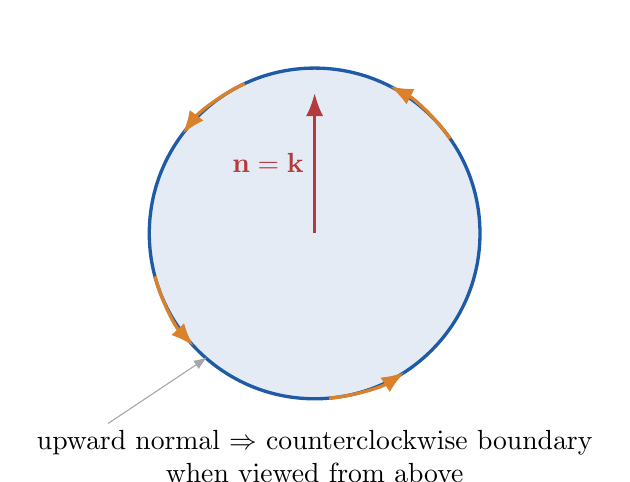
\begin{tikzpicture}[scale=2.1,>=Latex]
  \fill[chapterblue!12] (0,0) circle (1);
  \draw[very thick,chapterblue] (0,0) circle (1);
  \foreach \t in {35,115,195,275}{
    \draw[->,chapterorange,very thick] ({cos(\t)},{sin(\t)}) arc[start angle=\t,end angle=\t+28,radius=1];
  }
  \draw[->,very thick,chapterred] (0,0) -- (0,0.85) node[midway,left] {$\vn=\kk$};
  \node[align=center] at (0,-1.35) {upward normal $\Rightarrow$ counterclockwise boundary\\when viewed from above};
  \draw[->,gray!70] (-1.25,-1.15) -- (-0.65,-0.75);
\end{tikzpicture}
\caption{Boundary orientation for an upward oriented disk. Reversing the normal reverses the boundary direction.}
\end{figure}

For the disk in the $xy$-plane with upward normal $\vn=\kk$, the positive boundary orientation is counterclockwise when viewed from above. If the normal is changed to $-\kk$, the positive boundary orientation becomes clockwise.

\section{Stokes theorem}

\begin{theorembox}[Stokes theorem]
Let $S$ be an oriented smooth surface with boundary curve $C=\partial S$. Let $\vF$ be a vector field with continuous first partial derivatives near $S$. Then
\[
\oint_C \vF\cdot d\vr
=
\iint_S (\nabla\times\vF)\cdot\vn\,dS.
\]
\end{theorembox}

Here $C=\partial S$ is the boundary curve, $d\vr$ is tangent displacement along the curve, $\vF\cdot d\vr$ measures circulation, $\nabla\times\vF$ is the curl, and $(\nabla\times\vF)\cdot\vn$ measures the component of curl passing through the surface.

\begin{tipbox}[Surface independence]
If two oriented surfaces have the same boundary curve and compatible orientations, then Stokes theorem gives the same circulation integral over both surfaces. The boundary controls the answer.
\end{tipbox}

\section{Example: circulation around a circle}

\begin{examplebox}[Circulation around a circle]
Let
\[
\vF(x,y,z)=\langle -y,x,0\rangle.
\]
Let $C$ be the unit circle $x^2+y^2=1$, $z=0$, oriented counterclockwise as viewed from above. Parameterize
\[
\vr(t)=\langle \cos t,\sin t,0\rangle,\qquad 0\le t\le 2\pi.
\]
Then
\[
\vr'(t)=\langle -\sin t,\cos t,0\rangle,
\qquad
\vF(\vr(t))=\langle -\sin t,\cos t,0\rangle.
\]
Thus
\[
\vF(\vr(t))\cdot\vr'(t)=\sin^2t+\cos^2t=1,
\]
and
\[
\oint_C\vF\cdot d\vr=\int_0^{2\pi}1\,dt=2\pi.
\]
The curl is $\nabla\times\vF=\langle 0,0,2\rangle$. Using the unit disk with upward normal,
\[
\iint_S(\nabla\times\vF)\cdot\vn\,dS=\iint_S2\,dA=2\pi.
\]
The direct line integral and Stokes theorem agree.
\end{examplebox}

\begin{figure}[H]
\centering
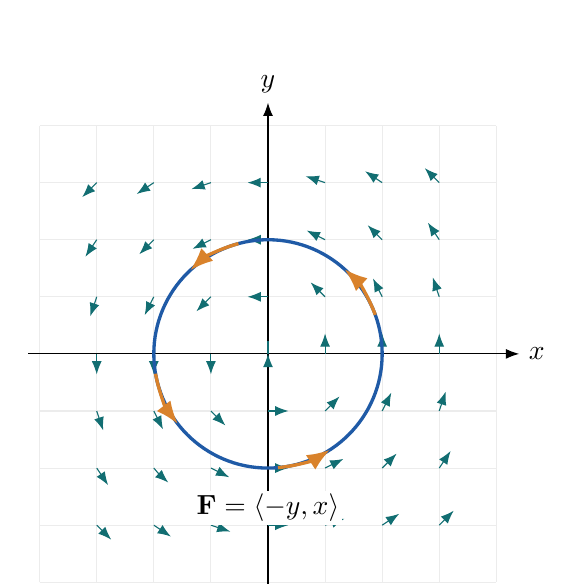
\begin{tikzpicture}[scale=1.45,>=Latex]
  \draw[step=0.5,gray!15] (-2,-2) grid (2,2);
  \draw[->] (-2.1,0) -- (2.2,0) node[right] {$x$};
  \draw[->] (0,-2.1) -- (0,2.2) node[above] {$y$};
  \foreach \x in {-1.5,-1,-0.5,0,0.5,1,1.5}{
    \foreach \y in {-1.5,-1,-0.5,0,0.5,1,1.5}{
      \pgfmathsetmacro{\m}{sqrt(\x*\x+\y*\y)+0.001}
      \pgfmathsetmacro{\u}{-0.18*\y/\m}
      \pgfmathsetmacro{\v}{0.18*\x/\m}
      \draw[->,chapterteal!80!black] (\x,\y) -- ++(\u,\v);
    }
  }
  \draw[very thick,chapterblue] (0,0) circle (1);
  \foreach \t in {20,105,190,275}{\draw[->,chapterorange,very thick] ({cos(\t)},{sin(\t)}) arc[start angle=\t,end angle=\t+28,radius=1];}
  \node[fill=white,inner sep=1pt] at (0,-1.35) {$\vF=\langle-y,x\rangle$};
\end{tikzpicture}
\caption{Rotational field and circulation around the unit circle. The field has constant upward curl $\langle0,0,2\rangle$.}
\end{figure}

\section{Stokes theorem as a computational shortcut}

Stokes theorem is useful in two directions. Sometimes the line integral is difficult but the curl integral is simple. Sometimes the surface integral is difficult but the boundary curve is simple. The theorem lets us choose the easier calculation.

\begin{examplebox}[Replacing a tilted surface by a flat disk]
Let
\[
\vF(x,y,z)=\langle -y,x,z\rangle.
\]
Let $S$ be any smooth oriented surface whose boundary is
\[
C:x^2+y^2=a^2,\qquad z=0,
\]
with upward-compatible orientation. The curl is still
\[
\nabla\times\vF=\langle 0,0,2\rangle.
\]
By Stokes theorem, instead of integrating over the possibly complicated surface $S$, we may use the flat disk $D$ bounded by $C$:
\[
\oint_C\vF\cdot d\vr=\iint_D2\,dA=2\pi a^2.
\]
The value depends on the boundary curve and orientation, not on the particular spanning surface.
\end{examplebox}

\begin{figure}[H]
\centering
\tdplotsetmaincoords{65}{115}
\begin{tikzpicture}[tdplot_main_coords,scale=2.15,>=Latex]
  \draw[->,gray!70] (-1.4,0,0) -- (1.5,0,0) node[below] {$x$};
  \draw[->,gray!70] (0,-1.4,0) -- (0,1.5,0) node[right] {$y$};
  \draw[->,gray!70] (0,0,-0.25) -- (0,0,0.9) node[above] {$z$};
  \filldraw[fill=chapterblue!12,draw=chapterblue,thick,opacity=0.8]
    plot[domain=0:360,samples=120] ({cos(\x)},{sin(\x)},{0}) -- cycle;
  \foreach \r in {0.25,0.5,0.75}{
    \draw[chapterblue!45] plot[domain=0:360,samples=90] ({\r*cos(\x)},{\r*sin(\x)},{0});
  }
  \draw[very thick,chapterorange] plot[domain=0:360,samples=160] ({cos(\x)},{sin(\x)},{0});
  \foreach \t in {20,120,220}{
    \draw[->,very thick,chapterorange] ({cos(\t)},{sin(\t)},0) -- ({cos(\t+18)},{sin(\t+18)},0);
  }
  \foreach \ang in {0,30,...,330}{
    \draw[chapterpurple!70,opacity=0.75] (0,0,0.34) -- ({cos(\ang)},{sin(\ang)},0);
  }
  \draw[chapterpurple,thick,dashed] plot[domain=0:360,samples=160] ({0.55*cos(\x)},{0.55*sin(\x)},{0.34*(1-0.55*0.55)*cos(2*\x)});
  \node[align=center,fill=white,inner sep=2pt] at (0,-1.45,0.15) {same boundary curve\\different spanning surfaces};
\end{tikzpicture}
\caption{Different spanning surfaces may share the same boundary curve. Stokes theorem lets us use the convenient one.}
\end{figure}

\section{Orientation signs in Stokes theorem}

Changing the orientation changes the sign. If $S$ has normal $\vn$, then
\[
\oint_{\partial S}\vF\cdot d\vr=\iint_S(\nabla\times\vF)\cdot\vn\,dS.
\]
If we reverse the normal to $-\vn$, then the boundary orientation also reverses, and both sides become negative:
\[
\oint_{-\partial S}\vF\cdot d\vr=\iint_S(\nabla\times\vF)\cdot(-\vn)\,dS.
\]
For $\vF=\langle-y,x,0\rangle$ on the unit circle, counterclockwise orientation gives $2\pi$, while clockwise orientation gives $-2\pi$.

\begin{figure}[H]
\centering
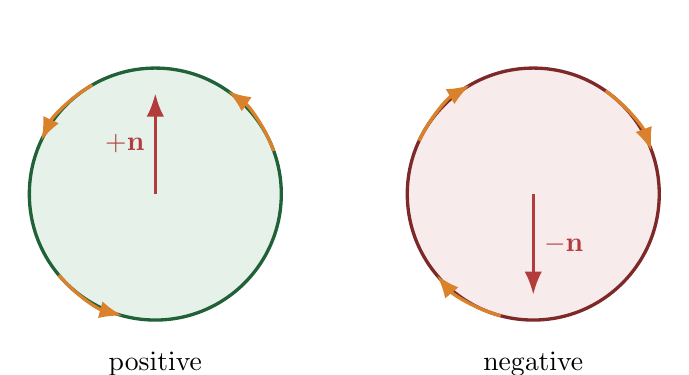
\begin{tikzpicture}[scale=1.6,>=Latex]
  \begin{scope}[xshift=-1.5cm]
  \fill[chaptergreen!12] (0,0) circle (1);
  \draw[very thick,chaptergreen!70!black] (0,0) circle (1);
  \foreach \t in {20,120,220}{\draw[->,chapterorange,very thick] ({cos(\t)},{sin(\t)}) arc[start angle=\t,end angle=\t+35,radius=1];}
  \draw[->,chapterred,very thick] (0,0) -- (0,0.8) node[midway,left] {$+\vn$};
  \node at (0,-1.35) {positive};
  \end{scope}
  \begin{scope}[xshift=1.5cm]
  \fill[chapterred!10] (0,0) circle (1);
  \draw[very thick,chapterred!70!black] (0,0) circle (1);
  \foreach \t in {20,120,220}{\draw[<-,chapterorange,very thick] ({cos(\t)},{sin(\t)}) arc[start angle=\t,end angle=\t+35,radius=1];}
  \draw[->,chapterred,very thick] (0,0) -- (0,-0.8) node[midway,right] {$-\vn$};
  \node at (0,-1.35) {negative};
  \end{scope}
\end{tikzpicture}
\caption{Reversing boundary orientation reverses the sign of circulation.}
\end{figure}

\section{The Divergence theorem}

\begin{theorembox}[The Divergence theorem]
Let $E$ be a solid region in $\R^3$ with closed boundary surface $\partial E$, oriented outward. If $\vF$ is a vector field with continuous first partial derivatives near $E$, then
\[
\iint_{\partial E}\vF\cdot\vn\,dS=\iiint_E\nabla\cdot\vF\,dV.
\]
\end{theorembox}

Here $\partial E$ is the closed boundary surface, $\vn$ is the outward unit normal, $\vF\cdot\vn$ measures outward flux density, $\nabla\cdot\vF$ measures local source strength, and the triple integral gives total source strength inside the solid.
\[
\text{outward flux through boundary}=\text{total divergence inside}.
\]

\begin{importantbox}[Closed surface required]
The Divergence theorem applies to a closed surface, meaning the full boundary of a solid. A single disk, a single hemisphere, or the side of a cylinder alone is not closed. If the surface is not closed, add the missing pieces or use a direct surface integral.
\end{importantbox}

\section{Example: flux through a sphere}

\begin{examplebox}[Outward radial field]
Let
\[
\vF(x,y,z)=\langle x,y,z\rangle.
\]
Let $S$ be the sphere $x^2+y^2+z^2=R^2$, oriented outward. On the sphere, the outward unit normal is
\[
\vn=\frac{1}{R}\langle x,y,z\rangle.
\]
Thus
\[
\vF\cdot\vn=\langle x,y,z\rangle\cdot\frac{1}{R}\langle x,y,z\rangle=\frac{x^2+y^2+z^2}{R}=R.
\]
Therefore
\[
\iint_S\vF\cdot\vn\,dS=\iint_SR\,dS=R(4\pi R^2)=4\pi R^3.
\]
The divergence is
\[
\nabla\cdot\vF=1+1+1=3.
\]
Hence
\[
\iint_S\vF\cdot\vn\,dS=\iiint_E3\,dV=3\cdot\frac{4\pi R^3}{3}=4\pi R^3.
\]
\end{examplebox}

\begin{figure}[H]
\centering
\tdplotsetmaincoords{68}{112}
\begin{tikzpicture}[tdplot_main_coords,scale=2.25,>=Latex]
  \shade[ball color=chapterblue!25,opacity=0.35] (0,0,0) circle (1);
  \draw[chapterblue!70!black,thick] (0,0,0) circle (1);
  \draw[chapterblue!55,dashed] (-1,0,0) arc[start angle=180,end angle=360,radius=1];
  \draw[chapterblue!70!black] plot[domain=0:360,samples=120] ({cos(\x)},{0},{sin(\x)});
  \foreach \p in {20,70,120,190,250,310}{
    \pgfmathsetmacro{\xx}{0.75*cos(\p)}
    \pgfmathsetmacro{\yy}{0.45*sin(\p)}
    \pgfmathsetmacro{\zz}{sqrt(max(0,1-\xx*\xx-\yy*\yy))}
    \draw[->,very thick,chapterred] (\xx,\yy,\zz) -- ({1.35*\xx},{1.35*\yy},{1.35*\zz});
  }
  \node[fill=white,inner sep=2pt] at (0,-1.35,0.2) {outward radial flux};
\end{tikzpicture}
\caption{Outward radial field on a sphere. For $\vF=\langle x,y,z\rangle$, every vector points normal to the sphere.}
\end{figure}

\section{Example: outward flux through a box}

\begin{examplebox}[Flux through a rectangular box]
Let
\[
\vF(x,y,z)=\langle x^2,y^2,z^2\rangle,
\qquad
E=[0,a]\times[0,b]\times[0,c].
\]
The divergence is
\[
\nabla\cdot\vF=2x+2y+2z.
\]
By the Divergence theorem,
\[
\iint_{\partial E}\vF\cdot\vn\,dS
=
\int_0^a\int_0^b\int_0^c(2x+2y+2z)\,dz\,dy\,dx.
\]
Computing term by term gives
\[
\iint_{\partial E}\vF\cdot\vn\,dS=a^2bc+ab^2c+abc^2=abc(a+b+c).
\]
For a unit cube, the answer is $3$.
\end{examplebox}

\begin{figure}[H]
\centering
\tdplotsetmaincoords{65}{120}
\begin{tikzpicture}[tdplot_main_coords,scale=2.1,>=Latex]
  \coordinate (O) at (0,0,0);
  \coordinate (A) at (1.6,0,0);
  \coordinate (B) at (1.6,1.1,0);
  \coordinate (C) at (0,1.1,0);
  \coordinate (D) at (0,0,0.9);
  \coordinate (E) at (1.6,0,0.9);
  \coordinate (F) at (1.6,1.1,0.9);
  \coordinate (G) at (0,1.1,0.9);
  \fill[chapterblue!10] (O)--(A)--(B)--(C)--cycle;
  \fill[chapterblue!18] (D)--(E)--(F)--(G)--cycle;
  \fill[chapterblue!14] (A)--(B)--(F)--(E)--cycle;
  \draw[thick] (O)--(A)--(B)--(C)--cycle (D)--(E)--(F)--(G)--cycle (O)--(D) (A)--(E) (B)--(F) (C)--(G);
  \foreach \x/\y/\z/\u/\v/\w in {0.8/0/0.45/0/-0.45/0,0.8/1.1/0.45/0/0.45/0,0/0.55/0.45/-0.45/0/0,1.6/0.55/0.45/0.45/0/0,0.8/0.55/0.9/0/0/0.45,0.8/0.55/0/0/0/-0.45}{
    \draw[->,very thick,chapterred] (\x,\y,\z) -- ++(\u,\v,\w);
  }
  \node[fill=white,inner sep=2pt] at (0.8,-0.35,0) {$E=[0,a]\times[0,b]\times[0,c]$};
\end{tikzpicture}
\caption{The Divergence theorem sums local source strength inside the box and equals outward flux through all six faces.}
\end{figure}

\section{Choosing the right theorem}

When a problem asks for a line integral, surface integral, circulation, or flux, choose the method that simplifies the geometry or lowers the dimension.

\begin{center}
\begin{tabularx}{\textwidth}{>{\bfseries}lX}
\toprule
Situation & Strategy\\
\midrule
Line integral over a curve & If the field is conservative, use a potential. If the curve is closed and bounds a surface, consider Stokes theorem. If it is planar, Green's theorem may be simpler.\\
Flux through a surface & If the surface is closed, consider the Divergence theorem. If it is open, add missing pieces or compute directly.\\
Curl through a surface & If the boundary curve is simple, use Stokes theorem. If the surface is simple, integrate directly.\\
Orientation uncertainty & Draw the normal and boundary direction before computing. Reversing orientation changes the sign.\\
\bottomrule
\end{tabularx}
\end{center}

\begin{tipbox}[Computational strategy]
Use the theorem that lowers the dimension or simplifies the geometry. A line integral may become a surface integral, a surface integral may become a triple integral, and a complicated surface may be replaced by a simpler surface with the same boundary.
\end{tipbox}

\section{Example: using Stokes theorem on a tilted triangle}

\begin{examplebox}[A triangular Stokes calculation]
Let
\[
\vF(x,y,z)=\langle y,z,x\rangle.
\]
Let $C$ be the boundary of the triangle with vertices
\[
A=(1,0,0),\qquad B=(0,1,0),\qquad C_0=(0,0,1),
\]
oriented so that the normal direction is compatible with
\[
\vn=\frac{1}{\sqrt3}\langle1,1,1\rangle.
\]
The curl is
\[
\nabla\times\vF
=\left\langle
\frac{\partial x}{\partial y}-\frac{\partial z}{\partial z},
\frac{\partial y}{\partial z}-\frac{\partial x}{\partial x},
\frac{\partial z}{\partial x}-\frac{\partial y}{\partial y}
\right\rangle
=\langle-1,-1,-1\rangle.
\]
The triangle lies in the plane $x+y+z=1$. Its oriented vector area is
\[
\frac12(B-A)\times(C_0-A)=\frac12\langle1,1,1\rangle.
\]
Therefore
\[
\oint_C\vF\cdot d\vr
=
\iint_S(\nabla\times\vF)\cdot\vn\,dS
=
\langle-1,-1,-1\rangle\cdot\frac12\langle1,1,1\rangle
=-\frac32.
\]
\end{examplebox}

\begin{figure}[H]
\centering
\tdplotsetmaincoords{70}{120}
\begin{tikzpicture}[tdplot_main_coords,scale=2.5,>=Latex]
  \coordinate (A) at (1,0,0);
  \coordinate (B) at (0,1,0);
  \coordinate (C) at (0,0,1);
  \coordinate (M) at (0.333,0.333,0.333);
  \draw[->,gray!70] (0,0,0) -- (1.2,0,0) node[below] {$x$};
  \draw[->,gray!70] (0,0,0) -- (0,1.2,0) node[right] {$y$};
  \draw[->,gray!70] (0,0,0) -- (0,0,1.2) node[above] {$z$};
  \filldraw[fill=chapterpurple!18,draw=chapterpurple,very thick] (A)--(B)--(C)--cycle;
  \draw[->,very thick,chapterorange] (A) -- ($(A)!0.18!(B)$);
  \draw[->,very thick,chapterorange] (B) -- ($(B)!0.18!(C)$);
  \draw[->,very thick,chapterorange] (C) -- ($(C)!0.18!(A)$);
  \draw[->,very thick,chapterred] (M) -- ++(0.38,0.38,0.38) node[above] {$\langle1,1,1\rangle$};
  \node[below] at (A) {$A$};
  \node[right] at (B) {$B$};
  \node[above] at (C) {$C_0$};
\end{tikzpicture}
\caption{Oriented triangular surface for a Stokes theorem calculation. The boundary orientation is chosen by the normal direction.}
\end{figure}

\section{Example: open surface plus missing cap}

\begin{examplebox}[Hemisphere with a disk cap]
Let
\[
\vF(x,y,z)=\langle x,y,z\rangle.
\]
Let $S$ be the upper hemisphere
\[
x^2+y^2+z^2=R^2,
\qquad z\ge 0,
\]
oriented outward. The hemisphere is not a closed surface. Add the disk
\[
D:x^2+y^2\le R^2,
\qquad z=0.
\]
The closed surface $S\cup D$ bounds the upper half-ball. By the Divergence theorem,
\[
\iint_{S\cup D}\vF\cdot\vn\,dS=\iiint_E3\,dV
=3\cdot\frac12\cdot\frac{4\pi R^3}{3}=2\pi R^3.
\]
On the disk $D$, the outward normal for the half-ball is $\vn=-\kk$, and $z=0$, so
\[
\vF\cdot\vn=\langle x,y,0\rangle\cdot\langle0,0,-1\rangle=0.
\]
Thus the flux through the upper hemisphere is
\[
\iint_S\vF\cdot\vn\,dS=2\pi R^3.
\]
For $R=1$, this is $2\pi$.
\end{examplebox}

\begin{figure}[H]
\centering
\tdplotsetmaincoords{70}{115}
\begin{tikzpicture}[tdplot_main_coords,scale=2.3,>=Latex]
  \fill[chaptergreen!12,opacity=0.75] plot[domain=0:360,samples=120] ({cos(\x)},{sin(\x)},{0}) -- cycle;
  \draw[chaptergreen!70!black,thick] plot[domain=0:360,samples=120] ({cos(\x)},{sin(\x)},{0});
  \foreach \a in {15,35,55,75}{
    \draw[chapterblue!50] plot[domain=0:360,samples=100] ({sin(\a)*cos(\x)},{sin(\a)*sin(\x)},{cos(\a)});
  }
  \foreach \t in {0,30,...,330}{
    \draw[chapterblue!45] (0,0,1) -- ({cos(\t)},{sin(\t)},0);
  }
  \draw[very thick,chapterblue] plot[domain=0:180,samples=100] ({cos(\x)},{0},{sin(\x)});
  \draw[->,very thick,chapterred] (0,0,0.55) -- (0,0,1.25) node[above] {hemisphere};
  \draw[->,very thick,chapterorange] (0.6,0.2,0) -- (0.6,0.2,-0.45) node[below] {cap normal};
\end{tikzpicture}
\caption{A hemisphere becomes a closed surface after adding its disk cap. The cap flux may be easier to compute.}
\end{figure}

\section{Numerical verification of Stokes theorem}

For $\vF=\langle-y,x,0\rangle$ and a circle of radius $R$, Stokes theorem predicts
\[
\oint_C\vF\cdot d\vr=2\pi R^2.
\]
A polygonal line-integral approximation converges to this value as the curve is refined.

\begin{figure}[H]
\centering
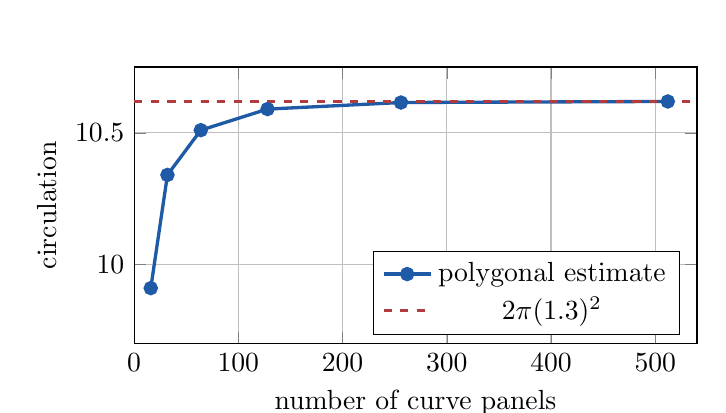
\begin{tikzpicture}
\begin{axis}[
  width=0.72\textwidth,
  height=0.42\textwidth,
  xlabel={number of curve panels},
  ylabel={circulation},
  grid=both,
  legend style={at={(0.97,0.03)},anchor=south east,fill=white},
  xmin=0,xmax=540,
  ymin=9.7,ymax=10.75
]
\addplot[very thick,mark=*,chapterblue] coordinates {(16,9.91) (32,10.34) (64,10.51) (128,10.59) (256,10.615) (512,10.619)};
\addlegendentry{polygonal estimate}
\addplot[very thick,dashed,chapterred] coordinates {(0,10.619) (540,10.619)};
\addlegendentry{$2\pi(1.3)^2$}
\end{axis}
\end{tikzpicture}
\caption{Numerical line-integral approximation agrees with Stokes theorem as the boundary curve approximation is refined.}
\end{figure}

\section{Numerical verification of the Divergence theorem}

For $\vF=\langle x,y,z\rangle$ and the unit ball, the Divergence theorem predicts
\[
\iint_S\vF\cdot\vn\,dS=\iiint_E3\,dV=4\pi.
\]
One can approximate the right side by Monte Carlo sampling inside the cube $[-1,1]^3$ and accepting points inside the unit ball.

\begin{figure}[H]
\centering
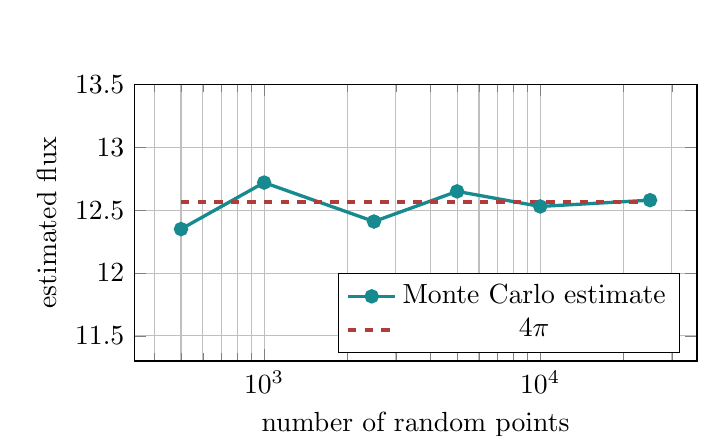
\begin{tikzpicture}
\begin{semilogxaxis}[
  width=0.72\textwidth,
  height=0.42\textwidth,
  xlabel={number of random points},
  ylabel={estimated flux},
  grid=both,
  legend style={at={(0.97,0.03)},anchor=south east,fill=white},
  ymin=11.3,ymax=13.5
]
\addplot[very thick,mark=*,chapterteal] coordinates {(500,12.35) (1000,12.72) (2500,12.41) (5000,12.65) (10000,12.53) (25000,12.58)};
\addlegendentry{Monte Carlo estimate}
\addplot[very thick,dashed,chapterred] coordinates {(500,12.566) (25000,12.566)};
\addlegendentry{$4\pi$}
\end{semilogxaxis}
\end{tikzpicture}
\caption{Monte Carlo estimate of total divergence inside the unit ball. Random estimates fluctuate but center near $4\pi$.}
\end{figure}

\section{Conservation laws and applied interpretation}

The Divergence theorem is the mathematical language of conservation laws. Suppose $\vF$ represents a flow field. Then:
\begin{itemize}
  \item $\vF\cdot\vn$ is the amount of flow crossing a boundary per unit area;
  \item $\iint_{\partial E}\vF\cdot\vn\,dS$ is the net flow leaving the region;
  \item $\nabla\cdot\vF$ is the local rate of expansion or source strength;
  \item $\iiint_E\nabla\cdot\vF\,dV$ is the total source strength inside.
\end{itemize}
If $\nabla\cdot\vF=0$, the field is incompressible or source-free. Then every closed surface has zero net outward flux:
\[
\iint_{\partial E}\vF\cdot\vn\,dS=0.
\]
This does not mean the field is zero. It means whatever flows into a closed region must also flow out.

\begin{figure}[H]
\centering
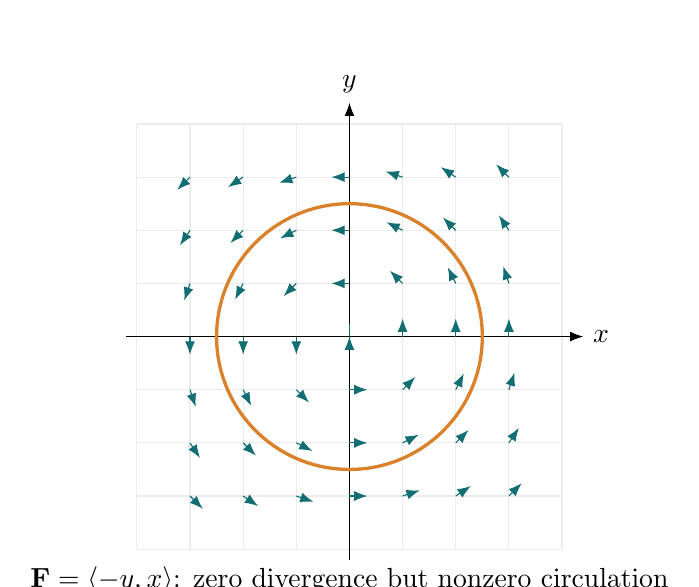
\begin{tikzpicture}[scale=1.35,>=Latex]
  \draw[step=0.5,gray!15] (-2,-2) grid (2,2);
  \draw[->] (-2.1,0) -- (2.2,0) node[right] {$x$};
  \draw[->] (0,-2.1) -- (0,2.2) node[above] {$y$};
  \foreach \x in {-1.5,-1,-0.5,0,0.5,1,1.5}{
    \foreach \y in {-1.5,-1,-0.5,0,0.5,1,1.5}{
      \pgfmathsetmacro{\m}{sqrt(\x*\x+\y*\y)+0.001}
      \pgfmathsetmacro{\u}{-0.17*\y/\m}
      \pgfmathsetmacro{\v}{0.17*\x/\m}
      \draw[->,chapterteal!80!black] (\x,\y) -- ++(\u,\v);
    }
  }
  \draw[very thick,chapterorange] (0,0) circle (1.25);
  \node[fill=white,inner sep=1pt] at (0,-2.3) {$\vF=\langle-y,x\rangle$: zero divergence but nonzero circulation};
\end{tikzpicture}
\caption{A rotational field can have zero divergence but nonzero curl. Divergence and curl measure different kinds of behavior.}
\end{figure}

\section{Summary of the four global theorems}

\begin{center}
\begin{tabularx}{\textwidth}{>{\bfseries}lXX}
\toprule
Theorem & Formula & Meaning\\
\midrule
Fundamental Theorem for Line Integrals & $\int_C\nabla f\cdot d\vr=f(B)-f(A)$ & gradient work depends only on endpoints\\
Green's theorem & $\oint_C P\,dx+Q\,dy=\iint_R(Q_x-P_y)\,dA$ & plane circulation equals total scalar curl\\
Stokes theorem & $\oint_{\partial S}\vF\cdot d\vr=\iint_S(\nabla\times\vF)\cdot\vn\,dS$ & boundary circulation equals total curl through surface\\
Divergence theorem & $\iint_{\partial E}\vF\cdot\vn\,dS=\iiint_E\nabla\cdot\vF\,dV$ & boundary flux equals total divergence inside\\
\bottomrule
\end{tabularx}
\end{center}

A good way to remember the pattern is
\[
\boxed{\text{boundary integral}=\text{interior integral of a derivative}.}
\]

\section{Common mistakes}

\begin{warningbox}[Common mistakes]
\begin{enumerate}
  \item \textbf{Using the Divergence theorem on an open surface.} The surface must be closed. If it is open, add missing pieces or compute directly.
  \item \textbf{Forgetting orientation.} Reversing orientation changes the sign of circulation or flux.
  \item \textbf{Mixing up curl and divergence.} Curl is a vector in three dimensions; divergence is a scalar.
  \item \textbf{Using Stokes theorem without a boundary curve.} A closed surface has no boundary, so Stokes theorem over a closed surface gives zero boundary circulation.
  \item \textbf{Forgetting surface replacement.} Any convenient surface with the same boundary and compatible orientation may be used.
  \item \textbf{Ignoring singularities.} The vector field must be sufficiently smooth on a region containing the surface or solid.
\end{enumerate}
\end{warningbox}

\section{Exercises}

\subsection*{Conceptual exercises}
\begin{enumerate}
  \item Explain the difference between circulation and flux.
  \item State Stokes theorem in words without using formulas.
  \item State the Divergence theorem in words without using formulas.
  \item Why does reversing the normal vector in Stokes theorem reverse the boundary orientation?
  \item Why does the Divergence theorem require a closed surface?
  \item Give an example of a vector field with zero divergence but nonzero curl.
  \item Give an example of a vector field with nonzero divergence but zero curl.
  \item Explain how Green's theorem is related to Stokes theorem.
\end{enumerate}

\subsection*{Computational exercises}
\begin{enumerate}
  \item Let $\vF=\langle-y,x,0\rangle$ and let $C$ be the circle $x^2+y^2=9$, $z=0$, oriented counterclockwise as viewed from above. Compute $\oint_C\vF\cdot d\vr$.
  \item Let $\vF=\langle y,z,x\rangle$ and let $S$ be the triangle with vertices $(1,0,0)$, $(0,1,0)$, and $(0,0,1)$, oriented by $\langle1,1,1\rangle$. Use Stokes theorem to compute $\oint_{\partial S}\vF\cdot d\vr$.
  \item Let $\vF=\langle x,y,z\rangle$ and let $S$ be the sphere of radius $2$ centered at the origin. Compute the outward flux through $S$.
  \item Let $\vF=\langle x^2,y^2,z^2\rangle$ and let $E=[0,2]\times[0,1]\times[0,3]$. Use the Divergence theorem to compute the outward flux through $\partial E$.
  \item Let $\vF=\langle yz,xz,xy\rangle$. Compute $\nabla\cdot\vF$. What does the Divergence theorem say about the outward flux through any closed surface?
  \item Let $\vF=\langle z,x,y\rangle$. Compute $\nabla\times\vF$ and use Stokes theorem over a convenient surface for a given circular boundary.
  \item Compute the outward flux of $\vF=\langle x,y,z\rangle$ through the upper hemisphere $x^2+y^2+z^2=4$, $z\ge0$.
  \item Use the Divergence theorem to compute the outward flux of $\vF=\langle x^3,y^3,z^3\rangle$ through the unit ball.
\end{enumerate}

\subsection*{Computational lab exercises}
\begin{enumerate}
  \item Modify the numerical Stokes theorem code for a circle of radius $R=2$ and compare with the exact value.
  \item Replace $\vF=\langle-y,x,0\rangle$ by $\vF=\langle-2y,3x,0\rangle$ and determine the new circulation around the unit circle.
  \item Use Monte Carlo sampling to estimate the flux of $\vF=\langle x,y,z\rangle$ through a ball of radius $2$.
  \item Write a function that estimates $\iiint_E\nabla\cdot\vF\,dV$ over a rectangular box using the midpoint rule.
  \item Visualize a vector field with zero divergence and nonzero curl.
  \item Visualize a vector field with nonzero divergence and zero curl.
\end{enumerate}

\section{Python lab and interactive page}

\begin{itemize}
  \item Notebook lab: \texttt{../labs/Chapter23\_Stokes\_Theorem\_and\_the\_Divergence\_Theorem.ipynb}
  \item Interactive HTML page: \texttt{../htmls/chapter-23.html}
\end{itemize}

\section{Chapter summary}

Stokes theorem and the Divergence theorem are global versions of differentiation. Stokes theorem says that circulation around a boundary equals total curl through a spanning surface. The Divergence theorem says that outward flux through a closed boundary equals total divergence inside the solid. Both theorems convert difficult boundary measurements into interior integrals, or difficult interior measurements into boundary integrals. Their common structure is the backbone of vector calculus and prepares students for conservation laws, partial differential equations, computational physics, geometric data analysis, and modern applied mathematics.

\end{document}
